\newcommand{\pluginName}{Dates Generator}
\newcommand{\pluginVersion}{1.0}


\input{../../../DocumentationTemplate/TemplateL3}

\begin{document}
\PluginTitle{\pluginName}{\pluginVersion}

\section{Introduction}
Dates generator allows to generate a sequence of (payment) dates by specifying Starting Date, Ending Date and the frequency.  Dates can then be manipolated manually and trasformed with adjustments.
\section{How to use the plug-in}
In the new symbol dialog window, a new symbol type is available.

After Dates Generator has been installed as a plugin from Settings $\to$ Plugins Settings 
$\to$ Available online plugins, you can then use it this way: 
\begin{enumerate}
\item Go to the Parameters \& Functions window
\item Click Add
\item Select Dates Generator and click Ok
\end{enumerate}
As you can see in the figure~\ref{fig:DG}, it is possible to set the start date and the end date setting also the desidered interval between each date entry (between these options: Daily, Weekly, Bi-Weekly, Montly, Three Months, Six Months, and Year).
\begin{figure}[h!]
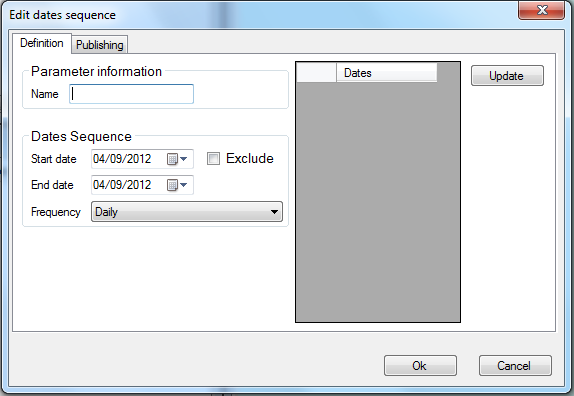
\includegraphics[width=4cm]{DG_img}
\centering
%\leftskip=-1.5 cm
\caption{\small{\emph{Dates Generator window.}}}
\label{fig:DG}
\end{figure}
The export option is used in Fairmat Server and Fairmat Professional to determine if the dates sequence will be shown from the interface and the templates. This procedure will make the Dates Generator manage the new parameter at all time. 

In case you want to be able to edit the output of the Dates Generator you'll have to follow a different procedure:
\begin{enumerate}
\item Go to the Parameters \& Functions window.
\item Click Add
\item Select Vector and click Ok
\item Give the new vector a name and close it by clicking Ok
\item Right click on the newly created vector and select Dates Generator
\item Set the start date, the ending date and the frequency, then press Ok
\end{enumerate}

This way the vector will be populated with all the dates as specified.



This new feature allows to build a vector of date directly in Fairmat avoiding the 
need of copying and pasting data from other software (i.e. from an Excel spreadsheet).

\end{document}
